%TC:ignore
\appendix
\chapter{Derivations}
\label{appen:derivations}
\section{Focused SAR Resolution}
\subsection{Along track resolution}
\begin{figure}
\centering
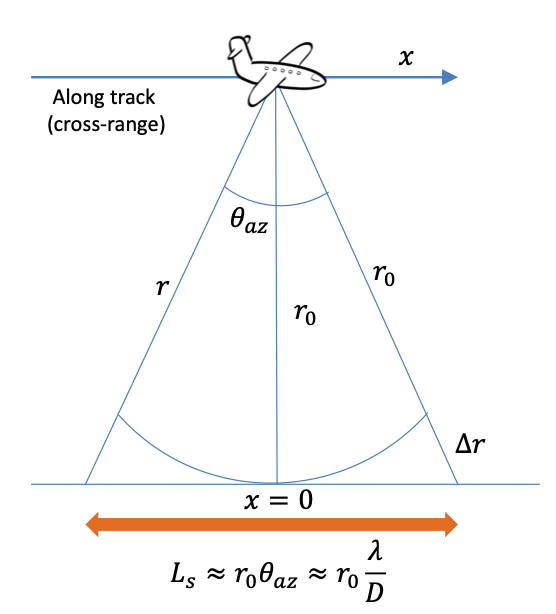
\includegraphics[width=0.5\linewidth]{../figures/sar_along_track_res}
\caption{Along-track/Cross-range SAR Resolution, reproduced from \cite{watsonEE40136RadarSystems2020}}
\label{fig:sar_along_track}
\end{figure}
\begin{gather}
	r = r_0 + \Delta r \\
	\Delta r = (r_0^2 + x^2) ^ \frac{1}{2} - r_0\\
	\Delta r \approx \frac{x^2}{2r_0}\\
	\phi(x) = -2k_0 \Delta r = -\frac{2\pi x^2}{\lambda r_0}\\
	\theta _{sa} \approx \frac{\lambda}{2L_s}\\
	\Delta x = \theta _{sa}r_0\\
	\Delta x = \frac{\lambda}{2L_s}r_0 = \frac{\lambda}{2r_0\frac{\lambda}{D}} r_0\\
	\Rightarrow \Delta x = \frac{D}{2}
\end{gather}
In this case, \gls{r} is the outer radial distance of the beam, \gls{r0} is the center distance of the beam, \gls{deltar} is the difference between these two distances, \gls{x} is the distance travelled by the platform over the time measured, \gls{k0} is the angular wave number of the signal, \gls{phix} is the two-way phase history of the signal, \gls{lambda} is the wavelength of the signal, \gls{thetasa} is the synthesised beam width obtained after azimuth processing, \gls{deltax} is the resolution of the system and \gls{D} is the aperture size in the chosen dimension (i.e. here it's the azimuthal dimension). Derivation from \cite{richardsRemoteSensingImaging2009} and \cite{watsonEE40136RadarSystems2020}.
\subsection{Down-range resolution}
\begin{figure}
\centering
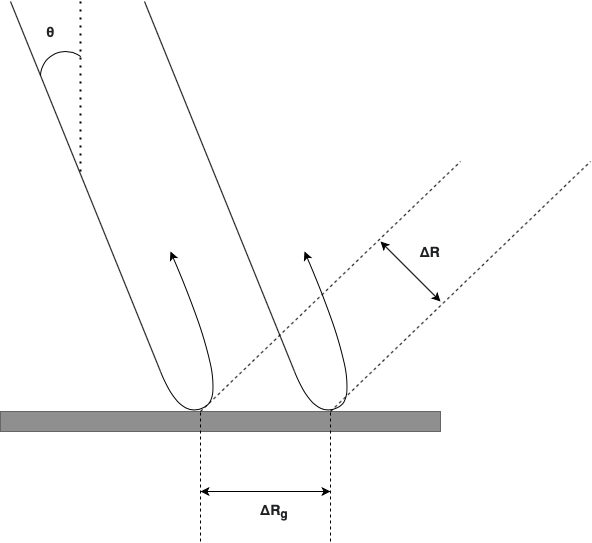
\includegraphics[width=0.5\linewidth]{../figures/down_range}	
\caption{Down-range SAR resolution, adapted from \cite{richardsRemoteSensingImaging2009}}
\label{fig:down_range_SAR}
\end{figure}
With the assumption made that there is some form of pulse compression on the signal we have a radial resolution of \[\Delta R = \frac{c}{2B}\] and by geometry we get a ground resolution of \[\Delta R_g = \frac{c}{2B\sin(\theta)}\] so to avoid any range ambiguities, \[\frac{c}{2R_{max}} > \text{PRF} \] where \gls{Rmax} is the maximum range achievable by the radar, \gls{DeltaRg} is the ground range resolution and \gls{DeltaR} is the radial resolution of the signal.
\section{Derivation of the Radar Equation}
Again derivations from \cite{richardsRemoteSensingImaging2009} and \cite{watsonEE40136RadarSystems2020}. \begin{gather}
 \text{Isotropic Antenna Power Density} = \frac{P_t}{4\pi R^2}\\
 \text{Directive Antenna Power Density} = \frac{P_tG_t}{4\pi R^2}\\
 \text{Power Intercepted by Target} = \frac{P_tG_t}{4\pi R^2}\sigma_b\\
 \text{Power density at receiver} = \frac{P_tG_T}{4\pi R^2}\sigma_b \times \frac{1}{4\pi R^2}\\
 P_r = \frac{P_tG_t}{4\pi R^2} \sigma_b \times \frac{1}{4\pi R^2} \times A_e \\
 G_r = \frac{4\pi}{\lambda^2}A_e\\
 G_t = G_r = G \\
 \Rightarrow P_r = \frac{P_tG^2\lambda^2}{(4\pi)^3R^4}\sigma_b
 \end{gather}
 Noise power \gls{Pn} is given by $P_n = kT_{sys}B$ and so the equation for SNR is given as \[ \frac{P_r}{P_n} = \frac{P_tG^2\lambda^2\sigma_b}{(4\pi)^3R^4kT_{sys}B}\] and so the radar equation for a distributed target is given by 
 \begin{gather}
 \sigma_b = \sigma^0 \Delta R_g \Delta x \\
 	\Delta x = \frac{R\lambda}{2L_s} = \frac{D}{2}\\
 	\Delta R_g = \frac{c}{2B\sin(90\degree - \alpha)}\\
 	t_{obs} = nT_s = \frac{L_s}{v_p}\\
 	n = \frac{L_s}{T_sv_p}\\
 	P_t = \frac{P_{av}T_s}{\tau}\\
 	\tau B \approx 1\\
 	\text{SNR}=\frac{P_{av}A_e^2\sigma^0\Delta R_g\Delta x t_{obs}}{4\pi\lambda^2kT_{sys}R^4} \text{or} \text{SNR} = \frac{P_{av}A_e^2\sigma^0\Delta x\lambda^3}{(4\pi)^3R^3kT_{sys}2v_p}
 \end{gather}





%TC:endignore